
\chapter{Small sample inference}
\label{smallSampleInference}

Large samples are sometimes unavailable, so it is useful to study methods that apply to small samples. Moving from large samples to small samples creates a number of problems that prevent us from applying the normal model directly, though the general ideas will be similar to those from Chapters~\ref{foundationsForInference} and~\ref{largeSampleInference}. The approach is as follows:
\begin{itemize}
\setlength{\itemsep}{0mm}
\item Determine what test statistic is useful.
\item Identify the distribution of the test statistic under the condition the null hypothesis was true.
\item Apply the ideas of Chapter~\ref{foundationsForInference} under the new distribution.
\end{itemize}
This is the same approach we used in Chapter~\ref{largeSampleInference}.
%It just so happened that the normal model worked very well for all the point estimates we studied when the sample size was large.

\section{Small sample inference for the mean}
\label{smallSampleInferenceForTheMean}

We applied a normal model to the sample mean in Chapter~\ref{foundationsForInference} when (1) the observations were independent, (2) the sample size was at least 50, and (3) the data were not strongly skewed. The findings in Section~\ref{cltSection} also suggested we could relax condition (3) when we considered ever larger samples.

In this section, we examine the distribution of the sample mean for any sample size. To this end, we must strengthen the condition about the distribution of the data. Specifically, our data must meet two criteria:
\begin{enumerate}
\item[(1)] The observations are independent.
\item[(2)] The population distribution is nearly normal.
\end{enumerate}
If we are not confident that the data come from a nearly normal distribution, then we cannot apply the methods of this section. Just like before, we can relax this condition when the sample size becomes larger.

Let's review our motives for requiring a large sample (for this paragraph, we will assume the independence and skew conditions are met). First, a large sample would ensure that the sampling distribution of the mean was nearly normal. Second, it also gave us support that the estimate of the standard error was reliable. Both of these issues seemed to be satisfactorily addressed when the sample size was larger than 50. Now, we'll think about how these issues (the shape of the sampling distribution, and the accuracy of the standard error estimate) change under small samples.

%It is useful to revisit our reasons for requiring a large sample for the normal model. We first wanted to ensure the sample mean was nearly normal. Secondly, when the sample size was small, the standard error estimate was not reliable. A sample size of 50 or more helps ensure this error estimate was adequate. We examine these two issues separately, leading us to a new distribution that will be useful for small sample inference about means.

\subsection{The normality condition}
\label{normalityCond}

If the individual observations are independent and come from a nearly normal population distribution, a special case of the Central Limit Theorem ensures the distribution of the sample means will be nearly normal.

\begin{termBox}{\tBoxTitle{Central Limit Theorem for normal data}
The sampling distribution of the mean is nearly normal when the sample observations are independent and come from a nearly normal distribution. This is true for any sample size.}
\end{termBox}

While this seems like a very helpful special case, there is one small problem. It is inherently difficult to verify normality in small data sets.

\begin{caution}
{Checking the normality condition}
{We should exercise caution when verifying the normality condition for small samples. It is important to not only examine the data but also think about where the data come from. For example, ask: would I expect this distribution to be symmetric, and am I confident that outliers are rare?}
%Always ask: Is it reasonable to assume this type of data are nearly normal?}
\end{caution}

%If we were to conduct simulations or investigate the mathematics, we would also find that we can relax our normality condition as the sample size becomes larger.


%Just as we could relax the concern of skew in Chapters~4 and~5 when the sample size became much larger, we will also find we can relax our restrictions on this normality assumption as the sample size becomes larger. For instance, if we have a sample of 15 observations and the data are symmetric and unimodal

\subsection{Introducing the $t$ distribution}

We will address the uncertainty of the standard error estimate by using a new distribution: the $t$ distribution. A $t$ distribution, shown as a solid line in Figure~\ref{tDistCompareToNormalDist}, has a bell shape. However, its tails are thicker than the normal model's. 
%This means we would not be as surprised to observe a random variable from the $t$ distribution further from zero than we would from a standard normal model (i.e. $N(0, 1)$).
This means observations are more likely to fall beyond two standard deviations from the mean than under the normal distribution\footnote{The standard deviation of the $t$ distribution is actually a little more than 1. However, it is useful to always think of the $t$ distribution as having a standard deviation of 1 in all of our applications.}.
These extra thick tails are exactly the correction we need to resolve our problem with estimating the standard error.
\begin{figure}
\centering
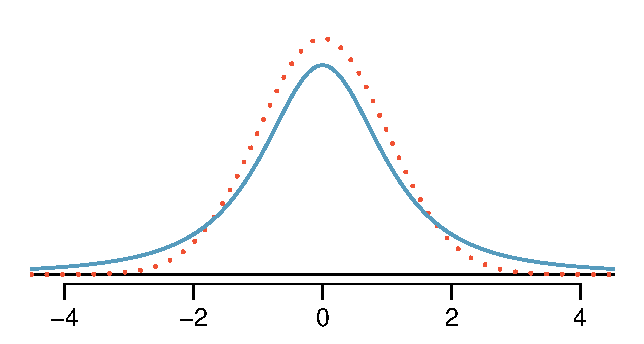
\includegraphics[height=45mm]{06/figures/tDistCompareToNormalDist/tDistCompareToNormalDist}
\caption{Comparison of a $t$ distribution (solid line) and a normal distribution (dotted line).}
\label{tDistCompareToNormalDist}
\end{figure}

%The normal model had two parameters: the mean ($\mu$) and the standard deviation ($\sigma$). 
The $t$ distribution, always centered at zero, has a single parameter: degrees of freedom. The \term{degrees of freedom ($\mathbf{df}$)} describe the exact bell shape of the $t$ distribution. Several $t$ distributions are shown in Figure~\ref{tDistConvergeToNormalDist}. When there are more degrees of freedom, the $t$ distribution looks very much like the standard normal distribution.
\begin{figure}
\centering
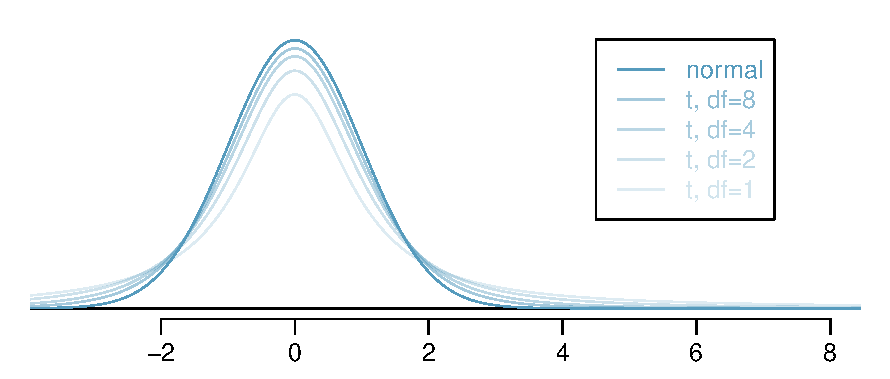
\includegraphics[width=0.7\textwidth]{06/figures/tDistConvergeToNormalDist/tDistConvergeToNormalDist}
\caption{The larger the degrees of freedom, the more closely the $t$ distribution resembles the standard normal model.}\vspace{-2mm}
\label{tDistConvergeToNormalDist}
\end{figure}

\begin{termBox}{\tBoxTitle{Degrees of freedom}
The degrees of freedom describe the shape of the $t$ distribution. The larger the degrees of freedom, the more closely the distribution approximates the normal model.}
\end{termBox}

When the degrees of freedom is about 50 or more, the $t$ distribution is nearly indistinguishable from the normal distribution. In Section~\ref{tDistSolutionToSEProblem}, we relate degrees of freedom to sample size.

\subsection{Working with the $t$ distribution}

We will find it very useful to become familiar with the $t$ distribution, because it plays a very similar role to the normal distribution during inference. We use a \term{t table} in place of the normal probability table, which is partially shown in Table~\ref{tTableSample}. A larger table is presented in Appendix~\vref{tDistributionTable}.
\begin{table}[hht]
\centering
\begin{tabular}{r | rrr rr}
one tail & \hspace{1.5mm}  0.100 & \hspace{1.5mm} 0.050 & \hspace{1.5mm} 0.025 & \hspace{1.5mm} 0.010 & \hspace{1.5mm} 0.005  \\
two tails & 0.200 & 0.100 & 0.050 & 0.020 & 0.010 \\
\hline
{$df$} \hfill 1  &  {\normalsize  3.08} & {\normalsize  6.31} & {\normalsize 12.71} & {\normalsize 31.82} & {\normalsize 63.66}  \\ 
2  &  {\normalsize  1.89} & {\normalsize  2.92} & {\normalsize  4.30} & {\normalsize  6.96} & {\normalsize  9.92}  \\ 
3  &  {\normalsize  1.64} & {\normalsize  2.35} & {\normalsize  3.18} & {\normalsize  4.54} & {\normalsize  5.84}  \\ 
$\vdots$ & $\vdots$ &$\vdots$ &$\vdots$ &$\vdots$ & \\
17  &  {\normalsize  1.33} & {\normalsize  1.74} & {\normalsize  2.11} & {\normalsize  2.57} & {\normalsize  2.90}  \\ 
\em\color{tableHLBlue}18  &  \em\color{tableHLBlue}{\normalsize  1.33} & \em\color{tableHLBlue}{\normalsize  1.73} & \em\color{tableHLBlue}{\normalsize  2.10} & \em\color{tableHLBlue}{\normalsize  2.55} & \em\color{tableHLBlue}{\normalsize  2.88}  \\ 
19  &  {\normalsize  1.33} & {\normalsize  1.73} & {\normalsize  2.09} & {\normalsize  2.54} & {\normalsize  2.86}  \\ 
20  &  {\normalsize  1.33} & {\normalsize  1.72} & {\normalsize  2.09} & {\normalsize  2.53} & {\normalsize  2.85}  \\ 
$\vdots$ & $\vdots$ &$\vdots$ &$\vdots$ &$\vdots$ & \\
400  &  {\normalsize  1.28} & {\normalsize  1.65} & {\normalsize  1.97} & {\normalsize  2.34} & {\normalsize  2.59}  \\ 
500  &  {\normalsize  1.28} & {\normalsize  1.65} & {\normalsize  1.96} & {\normalsize  2.33} & {\normalsize  2.59}  \\ 
$\infty$  &  {\normalsize  1.28} & {\normalsize  1.64} & {\normalsize  1.96} & {\normalsize  2.33} & {\normalsize  2.58}  \\ 
\end{tabular}
\caption{An abbreviated look at the $t$ table. Each row represents a different $t$ distribution. The columns describe the tail areas at each standard deviation. The row with $df=18$ has been {\em\color{tableHLBlue}highlighted}.}
\label{tTableSample}
\end{table}

Each row in the $t$ table represents a $t$ distribution with different degrees of freedom. The columns correspond to tail probabilities. For instance, if we know we are working with the $t$ distribution with $df=18$, we can examine row 18, which is highlighted in Table~\ref{tTableSample}. If we want the value in this row that identifies the cutoff for an upper tail of 10\%, we can look in the column where \emph{one tail} is 0.100. This cutoff is 1.33. If we had wanted the cutoff for the lower 10\%, we would use -1.33. Just like the normal distribution, all $t$ distributions are symmetric.

\begin{example}{What proportion of the $t$ distribution with 18 degrees of freedom falls below -2.10?}
Just like a normal probability problem, we first draw the picture in Figure~\ref{tDistDF18LeftTail2Point10} and shade the area below -2.10. To find this area, we identify the appropriate row: $df=18$. Then we identify the column containing the absolute value of -2.10; it is the third column. Because we are looking for just one tail, we examine the top line of the table, which shows that a one tail area for a value in the third row corresponds to 0.025. About 2.5\% of the distribution falls below -2.10. In the next example we encounter a case where the exact $t$ value is not listed in the table.
\end{example}
\begin{figure}
\centering
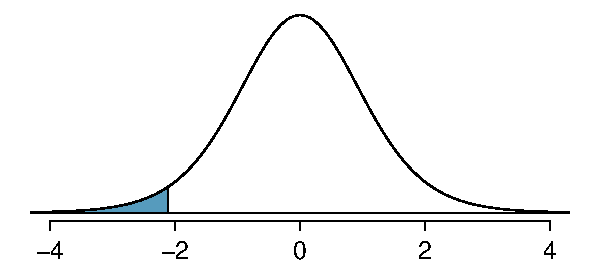
\includegraphics[width=0.51\textwidth]{06/figures/tDistDF18LeftTail2Point10/tDistDF18LeftTail2Point10}
\caption{The $t$ distribution with 18 degrees of freedom. The area below -2.10 has been shaded.}
\label{tDistDF18LeftTail2Point10}
\end{figure}

\begin{example}{A $t$ distribution with 20 degrees of freedom is shown in the left panel of Figure~\ref{tDistDF20RightTail1Point65}. Estimate the proportion of the distribution falling above 1.65.}
We identify the row in the $t$ table using the degrees of freedom: $df=20$. Then we look for 1.65; it is not listed. It falls between the first and second columns. Since these values bound 1.65, their tail areas will bound the tail area corresponding to 1.65. We identify the one tail area of the first and second columns, 0.050 and 0.10, and we conclude that between 5\% and 10\% of the distribution is more than 1.65 standard deviations above the mean. If we like, we can identify the precise area using statistical software: 0.0573.
\end{example}
\begin{figure}
\centering
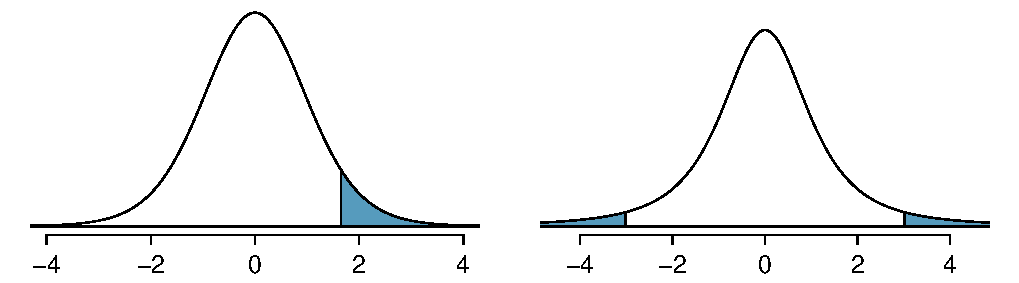
\includegraphics[width=0.85\textwidth]{06/figures/tDistDF20RightTail1Point65/tDistDF20RightTail1Point65}
\caption{Left: The $t$ distribution with 20 degrees of freedom, with the area above 1.65 shaded. Right: The $t$ distribution with 2 degrees of freedom, and the area further than 3 units from 0 has been shaded.}
\label{tDistDF20RightTail1Point65}
\end{figure}

\begin{example}{A $t$ distribution with 2 degrees of freedom is shown in the right panel of Figure~\ref{tDistDF20RightTail1Point65}. Estimate the proportion of the distribution falling more than 3 units from the mean (above or below).}
As before, first identify the appropriate row: $df=2$. Next, find the columns that capture 3; because $2.92 < 3 < 4.30$, we use the second and third columns. Finally, we find bounds for the tail areas by looking at the two tail values: 0.05 and 0.10. We use the two tail values because we are looking for two (symmetric) tails. %\footnote{From a computer: 0.0955.}.
\end{example}

\begin{exercise}
What proportion of the $t$ distribution with 19 degrees of freedom falls above -1.79 units? Answer in the footnote\footnote{We finding the shaded area \emph{above} -1.79 (we leave the picture to you). The small left tail is between 0.025 and 0.05, so the larger upper region must have an area between 0.95 and 0.975.}.
\end{exercise}

%The utility of the $t$ distribution is very much like that of the normal model. The primary differences are that we now must identify the degrees of freedom and the table has a different form.

%We investigate the influence of estimating the standard error in the context of hypothesis testing. We will perform this using a simulation since when we simulate we know everything about the data. \\

%\begin{exercise} \label{exerTestStatisticForHTWithNullMeanOf12AndUsingSampleSD}
%We would like to evaluate the following hypotheses:
%\begin{eqnarray*}
%H_0: \mu = 12 \\
%H_A: \mu \neq 12
%\end{eqnarray*}
%If we compute use the sample mean ($\bar{x}$), and we use the sample standard deviation, $s$, to estimate the standard error of the sample mean, $SE = s/\sqrt{n}$, what is the test statistic we use to evaluate the hypotheses? Answer in footnote\footnote{The point estimate of the population mean is $\bar{x}$, the null value for the mean is 12, and the standard error of our point estimate is $SE=s/\sqrt{n}$. Thus, we apply our test statistic formula: $t = \frac{\bar{x} - 12}{s/\sqrt{n}}$.}.
%\end{exercise}

%\begin{example}{We simulate our test statistic, $t$, from Exercise~\exer{exerTestStatisticForHTWithNullMeanOf12AndUsingSampleSD} when the sample size is 6. Each simulation represents a single sample of six observations with an unknown mean. Each observation is an independent observation from a normal distribution with mean 12. (We will reveal the actual standard deviation in a moment.) For each sample, sample mean, sample standard deviation, and test statistic were computed. The distribution of all 10,000 standard error estimates is shown in the left panel of Figure~\ref{distOfSEAndTestStatWhenSampleSizeIs6}, and the distribution of the test statistic is shown in the right panel.} \label{exampleSimulatingTestStatisticForHTWithNullMeanOf12AndUsingSampleSD}
%First examine the distribution of the estimated standard error. It is centered at the actual standard error, 5; the actual standard error was computed based on the standard deviation assigned in the simulation. While it is helpful that the estimate of standard error is centered at the true value, we also observe that the estimate is very volatile. For instance, it is not unusual to underestimate the standard error by 30\%!

%The right panel of Figure~\ref{distOfSEAndTestStatWhenSampleSizeIs6} shows the distribution of the test statistic. The best fitting normal curve is shown; this curve tends underestimate how often we observe test statistics far from 0. Had we used the normal model with this test statistic, we would have rejected the null hypothesis about 11\% of the time when using a $\alpha=5\%$ significance level (!).
%\end{example}
%\begin{figure}[hht]
%\centering
%%\includegraphics[height=2in]{06/figures/distOfSEAndTestStatWhenSampleSizeIs6/distOfSEAndTestStatWhenSampleSizeIs6}
%\caption{Estimates of the standard error based on the simulations performed in Example~\exam{exampleSimulatingTestStatisticForHTWithNullMeanOf12AndUsingSampleSD} are shown in the first panel. The actual standard error is 5. The second panel shows sample distribution of the test statistic when using the estimated standard errors. The normal model does not fit the distribution well in the tails, as shown in the third panel, which is a normal quantile plot of these test statistics.}
%\label{distOfSEAndTestStatWhenSampleSizeIs6}
%\end{figure}

%The distribution of the test statistic observed in the right panel of Figure~\ref{distOfSEAndTestStatWhenSampleSizeIs6} actually follows a completely new distribution: the \term{t distribution}\footnote{This distribution was identified near the start of the 20$^{th}$ century by William S. Gosset, a quality control engineer at Guinness Brewery in Dublin, Ireland. For good reason, Gosset opted to sample only a few drinks at a given time, at least while on the clock. Taking only small samples led him to identify issues in estimating the standard error when the sample size was small.}. The $t$ distribution is very much like the normal distribution except that it has thicker tails. That is, we are more likely to observe something far from the mean under the $t$ distribution rather than the normal distribution. A $t$ distribution representing the data in Example~\exam{exampleSimulatingTestStatisticForHTWithNullMeanOf12AndUsingSampleSD} is shown with a normal model in Figure~\ref{comparisonOfNormalAndTDist5DF}.
%\begin{figure}[hht]
%\centering
%%\includegraphics[height=2in]{06/figures/comparisonOfNormalAndTDist5DF/comparisonOfNormalAndTDist5DF}
%\caption{Comparison of the $t$ distribution with 5 degrees of freedom and the normal model.}
%\label{comparisonOfNormalAndTDist5DF}
%\end{figure}

%There are many $t$ distributions, just like there are many normal models. Different normal models might have different means or standard deviations. On the other hand, all $t$ distributions have mean 0 and standard deviation 1 differ by how thick their tails are. The parameter\footnote{Recall that parameters are numbers that define the characteristics of a distribution. For instance, the normal model parameters are the mean and standard deviation, $\mu$ and $\sigma$.} used to describe a $t$ distribution is \term{degrees of freedom (df)}.

%The degrees of freedom of the test statistics in Example~\exam{exampleSimulatingTestStatisticForHTWithNullMeanOf12AndUsingSampleSD} is 5. For a test statistic where the point estimate is the sample mean, the degrees of freedom is
%$$df = n-1$$
%where $n$ is the sample size. When the degrees of freedom are large, such as $df=49$, the $t$ distribution is almost identical to a normal distribution. This is consistent with our previous methods: when the sample size is at least 50, the normal model works well. Figure~\ref{comparisonOfNormalAndManyTDists} shows several $t$ distributions along with the normal model.
%\begin{figure}[hht]
%\centering
%%\includegraphics[height=2in]{06/figures/comparisonOfNormalAndManyTDists/comparisonOfNormalAndManyTDists}
%\caption{Comparison of several $t$ distributions and the normal model. As the sample size increases, so do degrees of freedom. For large sample size the $t$ distribution ends being very much like the normal model.}
%\label{comparisonOfNormalAndManyTDists}
%\end{figure}




%\subsection{Using the $t$ probability table}

\subsection{The $t$ distribution as a solution to the standard error problem}
\label{tDistSolutionToSEProblem}

When estimating the mean and standard error from a small sample, the $t$ distribution is a more accurate tool than the normal model.

\begin{tipBox}{\tipBoxTitle{When to use the $t$ distribution}
When observations are independent and nearly normal, we can use the $t$ distribution for inference of the sample mean.
}
\end{tipBox}

We use the $t$ distribution instead of the normal model because we have extra uncertainty in the estimate of the standard error. To proceed with the $t$ distribution for inference about a single mean, we must check two conditions.
\begin{itemize}
\item Independence of observations: We verify this condition exactly as before. We either collect a simple random sample from less than 10\% of the population or, if it was an experiment or random process, carefully ensure to the best of our abilities that the observations were independent.
\item Observations come from a nearly normal distribution: This second condition is more difficult to verify since we are usually working with small data sets. Instead we often (i) take a look at a plot of the data for obvious departures from the normal model and (ii) consider whether any previous experiences alert us that the data may not be nearly normal.
\end{itemize}
%As the sample size becomes larger, we may relax the normality condition. For instance, if the sample size is 50 or more, we can use the $t$ distribution with data so long as it is not extremely skewed. This actually replaces 
When examining a sample mean and estimated standard error from a sample of $n$ independent and nearly normal observations, we will use a $t$ distribution with $n-1$ degrees of freedom ($df$). For example, if the sample size was 19, then we would use the $t$ distribution with $df=19-1=18$ degrees of freedom and proceed exactly as we did in Chapter~\ref{foundationsForInference}, except that \emph{now we use the $t$ table}.

We can relax the normality condition for the observations when the sample size becomes large. For instance, a slightly skewed data set might be acceptable if there were at least 15 observations. For a strongly skewed data set, we might require 30 or 40 observations. For an extremely skewed data set, perhaps 100 or more.

\subsection{One sample confidence intervals with small $n$}

Dolphins are at the top of the oceanic food chain, which causes dangerous substances such as mercury to concentrate in their organs and muscles. This is an important problem for both dolphins and other animals, like humans, who occasionally eat them. For instance, this is particularly relevant in Japan where school meals have included dolphin at times.
\setlength{\captionwidth}{71.5mm}
\begin{figure}[h]
\centering
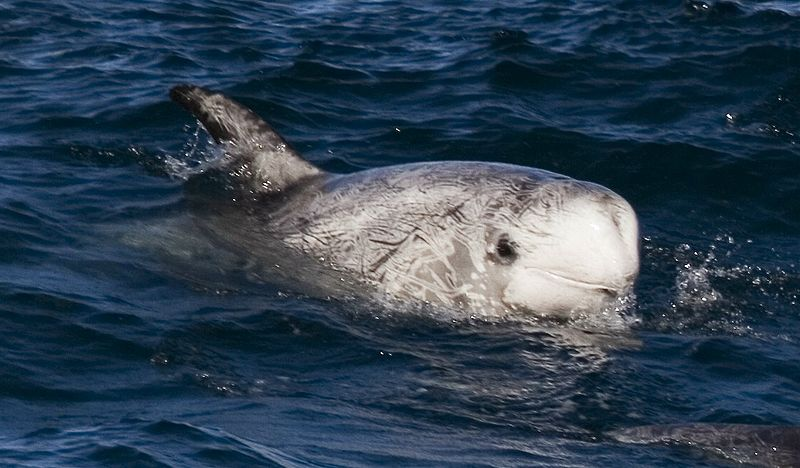
\includegraphics[width=71.5mm]{06/figures/rissosDolphin.jpg}  \\
\addvspace{2mm}
\begin{minipage}{\textwidth}
   \caption[rissosDolphinPic]{A Risso's dolphin.\vspace{-1mm} \\
   -----------------------------\vspace{-2mm}\\
   {\footnotesize Photo by Mike Baird (\urlwofont{http://www.bairdphotos.com/}).%Image is under Creative Commons Attribution 2.0 Generic.
}\vspace{-8mm}}
   \label{rissosDolphin}
\end{minipage}
\vspace{3mm}
%\begin{minipage}{\textwidth}
%\caption[rissosDolphinPic]{A Risso's dolphin\vspace{-3mm}\footnote{Photo by Mike Baird. Image is under Creative Commons Attribution 2.0 Generic.\vspace{2mm}}.}
%\end{minipage}
\end{figure}
\setlength{\captionwidth}{\mycaptionwidth}

Here we identify a confidence interval for the average mercury content in dolphin muscle using a sample of 19 Risso's dolphins from the Taiji area in Japan\footnote{Taiji was featured in the movie \emph{The Cove}, and it is a significant source of dolphin and whale meat in Japan. Thousands of dolphins pass through the Taiji area annually, and we will assume these 19 dolphins represent a random sample from those dolphins. Data reference: Endo T and Haraguchi K. 2009. High mercury levels in hair samples from residents of Taiji, a Japanese whaling town. Marine Pollution Bulletin 60(5):743-747.}. The data are summarized in Table~\ref{summaryStatsOfHgInMuscleOfRissosDolphins}. The minimum and maximum observed values can be used to evaluate whether or not there are any extreme outliers or obvious skew.
\begin{table}[h]
\centering
\begin{tabular}{ccc cc}
\hline
$n$ & $\bar{x}$ & $s$ & minimum & maximum \\
19   & 4.4	  & 2.3  & 1.7	       & 9.2 \\
\hline
\end{tabular}
\caption{Summary of mercury content in the muscle of 19 Risso's dolphins from the Taiji area. Measurements are in $\mu$g/wet g (micrograms of mercury per wet gram of muscle).}
\label{summaryStatsOfHgInMuscleOfRissosDolphins}
\end{table}

\begin{exercise}
%Evaluate the independence and normality conditions for applying the $t$ distribution to the sample mean and estimated standard error.
Are the independence and normality conditions satisfied for this data set? Answer in the footnote\footnote{The observations are a random sample and consist of less than 10\% of the population, therefore independence is reasonable. The summary statistics in Table~\ref{summaryStatsOfHgInMuscleOfRissosDolphins} do not suggest any strong skew or outliers, which is encouraging. Based on this evidence -- and that we don't have any clear reasons to believe the data are not roughly normal -- the normality assumption is reasonable.}.
\end{exercise}

In the normal model, we used $z^{\star}$ and the standard error to determine the width of a confidence interval. When we have a small sample, we try the $t$ distribution instead of the normal model:
\begin{eqnarray*}
\bar{x} \pm t^{\star}_{df}SE
\end{eqnarray*}
\marginpar[\raggedright\vspace{-9mm}

$t^{\star}_{df}$\vspace{1mm}\\\footnotesize Multiplication\\factor for\\$t$ conf. interval]{\raggedright\vspace{-9mm}

$t^{\star}_{df}$\vspace{1mm}\\\footnotesize Multiplication\\factor for\\$t$ conf. interval}The sample mean and estimated standard error are computed just as before ($\bar{x} = 4.4$ and $SE = s/\sqrt{n} = 0.528$), while the value $t^{\star}_{df}$ is a change from our previous formula. Here $t^{\star}_{df}$ corresponds to the appropriate cutoff from the $t$ distribution with $df$ degrees of freedom, which is identified below. 
%However, we must now identify $t^{\star}_{df}$ instead of $z^{\star}$ for the confidence interval.
%We first identify the degrees of freedom associated with the appropriate $t$ distribution (row $df=18$ in the $t$ table). Then determine the column corresponding to 95\% confidence (two tails: 0.05 for 95\% confidence). Then $t^{\star}_{df}$ is the intersection of this row and column in the $t$ table. 

\begin{termBox}{\tBoxTitle{Degrees of freedom for a single sample}
If our sample has $n$ observations and we are examining a single mean, then we use the $t$ distribution with $df=n-1$ degrees of freedom.}
\end{termBox}

Applying the rule in our current example, we should use the $t$ distribution with $df=19-1=18$ degrees of freedom. To build a 95\% confidence interval, we will use the abbreviated $t$ table on page~\pageref{tTableSample} where each tail has 2.5\% (both tails total to 5\%), which is the third column. Then we identify the row with 18 degrees of freedom to obtain $t^{\star}_{18} = 2.10$. Generally the value of $t^{\star}_{df}$ is slightly larger than what we would expect under the normal model with $z^{\star}$.



Finally, we can substitute all our values into the confidence interval equation to create the 95\% confidence interval for the average mercury content in muscles from Risso's dolphins that pass through the Taiji area:
\begin{eqnarray*}
\bar{x} \pm t^{\star}_{18}SE
	\quad \to \quad
4.4 \pm 2.10 * 0.528
	\quad \to \quad
(3.87, 4.93)
\end{eqnarray*}
We are 95\% confident the average mercury content of muscles in Risso's dolphins is between 3.87 and 4.93 $\mu$g/wet gram. This falls below the US safety limit, which is 0.5 $\mu$g per wet gram\footnote{http://www.ban.org/ban-hg-wg/Mercury.ToxicTimeBomb.Final.PDF}.  %EPA's recommended dose of mercury for a day is 0.1 micrograms mercury per kilogram body weight (of the person eating the food); eating about 2 grams of the ``average'' Risso's dolphin meat would put a 150 lb person above the recommended mercury dose for the day (!).  

\begin{termBox}{\tBoxTitle{Finding a $t$ confidence interval for the mean}
Based on a sample of $n$ independent and nearly normal observations, a confidence interval for the population mean is
$$\bar{x} \pm t^{\star}_{df}SE$$
where $\bar{x}$ is the sample mean, $t^{\star}_{df}$ corresponds to the confidence level and degrees of freedom, and $SE$ is the standard error as estimated by the sample.}
\end{termBox}

\begin{exercise} \label{croakerWhiteFishPacificExerConditions}
The FDA's webpage provides some data on mercury content of fish\footnote{http://www.fda.gov/Food/FoodSafety/Product-SpecificInformation/Seafood/\\ FoodbornePathogensContaminants/Methylmercury/ucm115644.htm}. Based on a sample of 15 croaker white fish (Pacific), a sample mean and standard deviation were computed as 0.287 and 0.069 ppm (parts per million), respectively. The 15 observations ranged from 0.18 to 0.41 ppm. We will assume these observations are independent. Based on the summary statistics of the data, do you have any objections to the normality condition of the individual observations? Answer in the footnote\footnote{There are no extreme outliers; all observations are within 2 standard deviations of the mean. If there is skew, it is not evident. There are no red flags for the normal model based on this (limited) information, and we do not have reason to believe the mercury content is not nearly normal in this type of fish.}.
\end{exercise}

%ZZQ Formatting
\vspace{5mm}

\begin{example}{Estimate the standard error of $\bar{x}=0.287$ ppm from the statistics in Exercise~\exer{croakerWhiteFishPacificExerConditions}. If we are to use the $t$ distribution to create a 90\% confidence interval for the actual mean of the mercury content, identify the degrees of freedom we should use and also find $t^{\star}_{df}$.}
\label{croakerWhiteFishPacificExerSEDFTStar}
$SE = \frac{0.069}{\sqrt{15}} = 0.0178$ and $df = n - 1 = 14$. Looking in the column where two tails is 0.100 (since we want a 90\% confidence interval) and row $df=14$, we identify $t^{\star}_{14} = 1.76$.
\end{example}

\begin{exercise}
Based on the results of Exercise~\exer{croakerWhiteFishPacificExerConditions} and Example~\exam{croakerWhiteFishPacificExerSEDFTStar}, compute a 90\% confidence interval for the average mercury content of croaker white fish (Pacific). Answer in the footnote\footnote{Use $\bar{x} \pm t^{\star}_{14} SE$: $0.287 \pm 1.76*0.0178$. This corresponds to $(0.256, 0.318)$. We are 90\% confident that the average mercury content of croaker white fish (Pacific) is between 0.256 and 0.318 ppm.}.
\end{exercise}

\subsection{One sample $t$ tests with small $n$}

An SAT preparation company claims that its students' scores improve by over 100 points on average after their course. A consumer group would like to evaluate this claim, and they collect data on a random sample of 30 students who took the class. Each of these students took the SAT before and after taking the company's course, and we would like to examine the differences in these scores to evaluate the company's claim. (This was originally paired data, so we use the differences; see Section~\ref{pairedData} for more details on paired data.)
 The distribution of the difference in scores, shown in Figure~\ref{satImprovementHTDataHistogram}, has mean 135.9 and standard deviation 82.2. Do these data provide convincing evidence to back up the company's claim? 
\begin{figure}
\centering
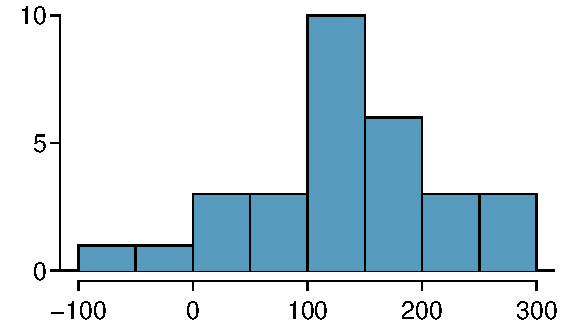
\includegraphics[width=0.54\textwidth]{06/figures/satImprovementHTDataHistogram/satImprovementHTDataHistogram}
\caption{Sample distribution of improvements in SAT scores after taking the SAT course.}
\label{satImprovementHTDataHistogram}
\end{figure}

\begin{exercise}
Set up hypotheses to evaluate the company's claim. Use $\mu$ to represent the true average difference in student scores. Answer in the footnote\footnote{This is a one-sided test. $H_0$: student scores do not improve by more than 100 after taking the company's course. $\mu \leq 100$ (or simply $\mu = 100$). $H_A$: students scores improve by more than 100 points on average after taking the company's course. $\mu > 100$.}.
\end{exercise}

\begin{exercise}
Are the conditions to use the $t$ distribution method satisfied? Answer in the footnote\footnote{This is a random sample from less than 10\% of the company's students (assuming they have more than 300 former students), so the independence condition is reasonable. The normality condition also seems reasonable based on Figure~\ref{satImprovementHTDataHistogram}. We can use the $t$ distribution method.}.
\end{exercise}

Just as we did for the normal case, we standardize the sample mean using the Z score to identify the test statistic. However, we will write $T$\marginpar[\raggedright$T$\vspace{0.5mm}\\\footnotesize T score\\(like Z score)]{\raggedright$T$\vspace{0.5mm}\\\footnotesize T score\\(like Z score)} instead of $Z$, because we have a small sample and are basing our inference on the $t$ distribution:
%However, because we have a small sample and will use the $t$ distribution for the test statistic, we will label the standardized mean with $T$ instead of $Z$:
\begin{eqnarray*}
T = \frac{\bar{x} - \text{null value}}{SE} = \frac{135.9 - 100}{82.2/\sqrt{30}} = 2.39
\end{eqnarray*}
If the null hypothesis was true, the test statistic $T$ would follow a $t$ distribution with $df = n-1 = 29$ degrees of freedom. We can draw a picture of this distribution and mark the observed $T$, as in Figure~\ref{pValueShownForSATHTOfOver100PtGain}. The shaded right tail represents the p-value: the probability of observing such strong evidence in favor of the SAT company's claim, if the average student improvement is really only 100.
\begin{figure}
\centering
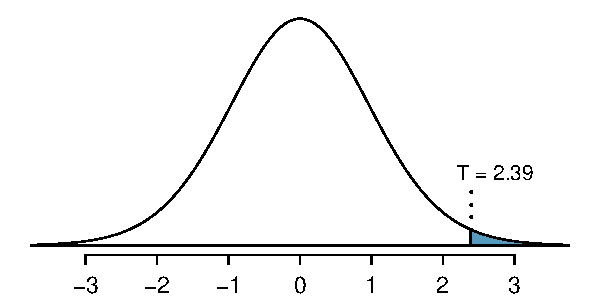
\includegraphics[width=0.65\textwidth]{06/figures/pValueShownForSATHTOfOver100PtGain/pValueShownForSATHTOfOver100PtGain}
\caption{The $t$ distribution with 29 degrees of freedom.}
\label{pValueShownForSATHTOfOver100PtGain}
\end{figure}

\begin{exercise}
Use the $t$ table in Appendix~\vref{tDistributionTable} to identify the p-value. What do you conclude? Answer in the footnote\footnote{We use the row with 29 degrees of freedom. The value $T=2.39$ falls between the third and fourth columns. Because we are looking for a single tail, this corresponds to a p-value between 0.01 and 0.025. The p-value is guaranteed to be less than 0.05 (the default significance level), so we reject the null hypothesis. The data provide convincing evidence to support the company's claim that student scores improve by more than 100 points following the class.}.
\end{exercise}

\begin{exercise}
Because we rejected the null hypothesis, does this mean that taking the company's class improves student scores by more than 100 points on average? Answer in the footnote\footnote{This is an observational study, so we cannot make this causal conclusion. For instance, maybe SAT test takers tend to improve their score over time even if they don't take a special SAT class, or perhaps only the most motivated students take such SAT courses.}.
\end{exercise}

\section{The $t$ distribution for the difference of two means}

It is useful to be able to compare two means. For instance, a teacher might like to test the notion that two versions of an exam were equally difficult. She could do so by randomly assigning each version to students. If she found that the average scores on the exams were so different that we cannot write it off as chance, then she may want to award extra points to students who took the more difficult exam.

In a medical context, we might investigate whether embryonic stem cells (ESCs) can improve heart pumping capacity in individuals who have suffered a heart attack. We could look for evidence of greater heart health in the ESC group against a control group. % We compare this group to a control group that suffered heart attacks but did not receive ESCs. We will find it useful to evaluate whether the evidence convincingly shows that sheep in the ESC group have more improvement than sheep in the control group on average.

The ability to make conclusions about a difference in two means, $\mu_1 - \mu_2$, is often useful. If the sample sizes are small and the data are nearly normal, the $t$ distribution can be applied to the sample difference in means, $\bar{x}_1 - \bar{x}_2$, to make inference about the difference in population means.

\subsection{Sampling distributions for the difference in two means}

In the example of two exam versions, the teacher would like to evaluate whether there is convincing evidence that the difference in average scores is not due to chance.
% Similarly, we might like to evaluate whether the difference in pumping capacity of the ESC and control groups provides convincing evidence that stem cells actually do help improve heart function following a heart attack.

It will be useful to extend the $t$ distribution method from Section~\ref{smallSampleInferenceForTheMean} to apply to a new point estimate:
\begin{eqnarray*}
\bar{x}_1 - \bar{x}_2
\end{eqnarray*}
Just as we did in Section~5.2, %ZZQ \ref{}, 
we verify conditions for each sample separately and then verify that the samples are also independent. For instance, if the teacher believes students in her class are independent, the exam scores are nearly normal, and the students taking each version of the exam were independent, then we can use the $t$ distribution for the sampling distribution of the point estimate, $\bar{x}_{1} - \bar{x}_{2}$.

The formula for the standard error of $\bar{x}_{1} - \bar{x}_{2}$, introduced in Section~5.2,  %ZZQ \ref{},
remains useful for small samples:
\begin{eqnarray}
SE_{\bar{x}_1 - \bar{x}_2}
	= \sqrt{SE_{\bar{x}_1}^2 + SE_{\bar{x}_2}^2}
	 = \sqrt{\frac{s_1^2}{n_1} + \frac{s_2^2}{n_2}} \label{seOfDiffOfTwoMeansInTDistSection}
\end{eqnarray}
Because we will use the $t$ distribution, we will need to identify the appropriate degrees of freedom. This can be done using computer software. An alternative technique is to use the smaller of $n_1 - 1$ and $n_2 - 1$, which is the method we will apply in the examples and exercises\footnote{This technique for degrees of freedom is conservative with respect to a Type 1 Error; it is more difficult to reject the null hypothesis using this $df$ method.}. 

\begin{termBox}{\tBoxTitle{Using the $t$ distribution for a difference in means}
The $t$ distribution can be used for the (standardized) difference of two means if (1) each sample meets the conditions for the $t$ distribution and (2) the samples are independent. We estimate the standard error of the difference of two means using Equation~(\ref{seOfDiffOfTwoMeansInTDistSection}).}
\end{termBox}

%In this section, we apply the same $t$ distribution methods of Section~\ref{smallSampleInferenceForTheMean} to the point estimate of the difference in means: $\bar{x}_1 - \bar{x}_2$.

\subsection{Two sample $t$ test}
%Do not include the test with pooled standard deviations are grouped but mention it as one method that is discussed in other books.% (I consider this to be a poor test -- if the sd's are remotely similar then the result will be basically the same as the sd's are not assumed to be the same... seems like a big assumption that can results in too many problems with almost no benefits.)

%Two versions of an exam were given out to students to reduce cheating. However, when the professor examined the average scores on the two exams, she saw that they were different. 
Summary statistics for each exam version are shown in Table~\ref{summaryStatsForTwoVersionsOfExams}. The teacher would like to evaluate whether this difference is so large that it provides convincing evidence that Version B was more difficult (on average) than Version A. 
\begin{table}[hht]
\centering
\begin{tabular}{l rrrrr}
\hline
Version\hspace{2mm}	& $n$	& $\bar{x}$	& $s$	& min	& max  \\
\hline
A		& 30		& 79.4		& 14 	& 45		& 100 \\
B		& 27		& 74.1		& 20		& 32		& 100 \\
\hline
\end{tabular}
\caption{Summary statistics of scores for each exam version.}
\label{summaryStatsForTwoVersionsOfExams}
\end{table}

\begin{exercise} \label{htSetupForEvaluatingTwoExamVersions}
Construct a two-sided hypothesis test to evaluate whether the observed difference in sample means, $\bar{x}_A - \bar{x}_B=5.3$, might be due to chance. Answer in the footnote\footnote{Because the professor did not expect one exam to be more difficult prior to examining the test results, she should use a two-sided hypothesis test. $H_0$: the exams are equally difficult, on average. $\mu_A - \mu_B = 0$. $H_A$: one exam was more difficult than the other, on average. $\mu_A - \mu_B \neq 0$.}.
\end{exercise}

\begin{exercise} \label{conditionsForTDistForEvaluatingTwoExamVersions}
To evaluate the hypotheses in Exercise~\exer{htSetupForEvaluatingTwoExamVersions} using the $t$ distribution, we must first verify assumptions. (a) Does it seem reasonable that the scores are independent? (b) What about the normality condition for each group? (c) Do you think each group would be independent? Answer in the footnote\footnote{(a) It is probably reasonable to conclude the scores are independent. (b) The summary statistics suggest the data are roughly symmetric about the mean, and it doesn't seem unreasonable to suggest the data might be normal. (c) It seems reasonable to suppose that the samples are independent since the exams were handed out randomly.}.
\end{exercise}

After verifying the conditions for each sample and confirming the samples are independent of each other, we are ready to conduct the test using the $t$ distribution. In this case, we are estimating the true difference in average test scores using the sample data, so the point estimate is $\bar{x}_A - \bar{x}_B = 5.3$. The standard error of the estimate can be calculated using Equation~(\ref{seOfDiffOfTwoMeansInTDistSection}):
\begin{eqnarray*}
SE = \sqrt{\frac{s_A^2}{n_A} + \frac{s_B^2}{n_B}} = \sqrt{\frac{14^2}{30} + \frac{20^2}{27}} = 4.62
\end{eqnarray*}
Finally, we construct the test statistic:
\begin{eqnarray*}
T = \frac{\text{point estimate} - \text{null value}}{SE} = \frac{(79.4-74.1) - 0}{4.62} = 1.15
\end{eqnarray*}
If we have a computer handy, we can identify the degrees of freedom as 45.97. Otherwise we use the smaller of $n_1-1$ and $n_2-1$: $df=26$. 
\begin{figure}
\centering
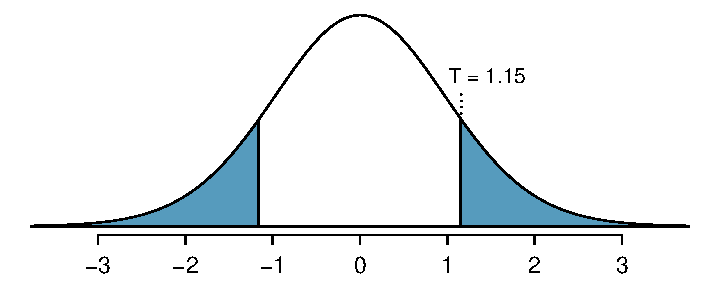
\includegraphics[width=0.65\textwidth]{06/figures/pValueOfTwoTailAreaOfExamVersionsWhereDFIs26/pValueOfTwoTailAreaOfExamVersionsWhereDFIs26}
\caption{The $t$ distribution with 26 degrees of freedom. The shaded right tail represents values with $T \geq 1.15$. Because it is a two-sided test, we also shade the corresponding lower tail.}
\label{pValueOfTwoTailAreaOfExamVersionsWhereDFIs26}
\end{figure}

\begin{exercise} \label{computeTwoTailAreaOfExamVersionsWhereDFIs26}
Identify the p-value, shown in Figure~\ref{pValueOfTwoTailAreaOfExamVersionsWhereDFIs26}. Use $df=26$. Answer in the footnote\footnote{We examine row $df=26$ in the $t$ table. Because this value is smaller than the value in the left column, the p-value is at least 0.200 (two tails!). Because the p-value is so large, we do not reject the null hypothesis. That is, the data do not convincingly show that one exam version is more difficult than the other, and the teacher is not convinced that she should add points to the Version B exam scores.}.
\end{exercise}

In Exercise~\exer{computeTwoTailAreaOfExamVersionsWhereDFIs26}, we could have used $df=45.97$. However, this value is not listed in the table. In such cases, we use the next lower degrees of freedom (unless the computer also provides the p-value). For example, we could have used $df=45$ but not $df=46$. 

Do embryonic stem cells (ESCs) help improve heart function following a heart attack? Table~\ref{summaryStatsForSheepHeartDataWhoReceivedMiceESCs} contains summary statistics for an experiment to test ESCs in sheep that had a heart attack. Each of these sheep was randomly assigned to the ESC or control group, and the change in their hearts' pumping capacity was measured. A positive value generally corresponds to increased pumping capacity, which suggests a stronger recovery. We will consider this study in the exercises and examples below.

\begin{exercise} \label{exerciseToEvaluteWhetherESCsAreHelpfulInImprovingHeartFunctionInSheep}
Set up hypotheses that will be used to test whether there is convincing evidence that ESCs actually increase the amount of blood the heart pumps. Answer in the footnote\footnote{We first setup the hypotheses:
\begin{itemize}
\item[$H_0$:] The stem cells do not improve heart pumping function. $\mu_{esc} - \mu_{control} = 0$.
\item[$H_A$:] The stem cells do improve heart pumping function. $\mu_{esc} - \mu_{control} > 0$.
\end{itemize}
Before we move on, we must first verify that the $t$ distribution method can be applied. Because the sheep were randomly assigned their treatment and, presumably, were kept separate from one another, the independence assumption is verified for each sample as well as for between samples. The data are very limited, so we can only check for obvious outliers in the raw data in Figure~\ref{stemCellTherapyForHearts}. Since the distributions are (very) roughly symmetric, we will assume the normality condition is acceptable. Because the conditions are satisfied, we can apply the $t$ distribution.}.
\end{exercise}
\begin{table}
\centering
\begin{tabular}{l rrrrr}
\hline
\hspace{10mm}	& $n$	& $\bar{x}$	& $s$  	 \\
\hline
ESCs		& 9		& 3.50		& 5.17  	\\
control		& 9		& -4.33		& 2.76  	 \\
\hline
\end{tabular}
\caption{Summary statistics of scores, split by exam version.}
\label{summaryStatsForSheepHeartDataWhoReceivedMiceESCs}
\end{table}
\begin{figure}
\centering
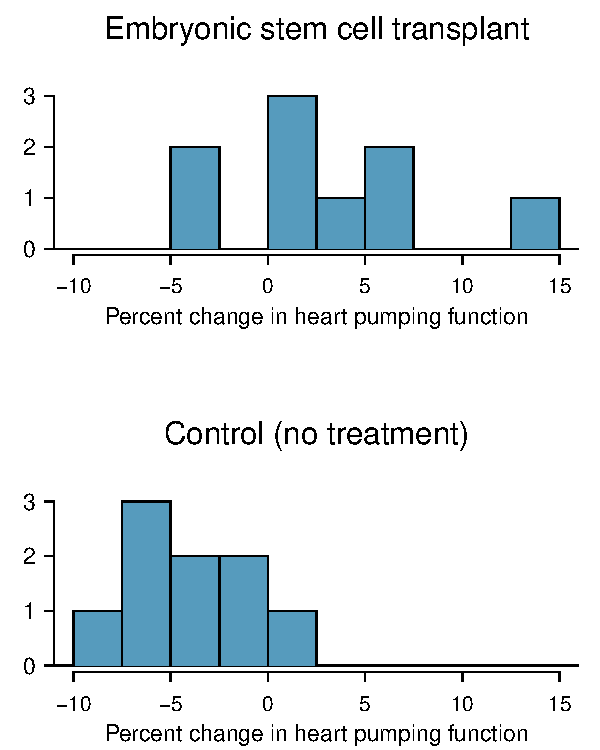
\includegraphics[width=0.6\textwidth]{06/figures/stemCellTherapyForHearts/stemCellTherapyForHearts}
\caption{Histograms for both the embryonic stem cell group and the control group. Higher values are associated with greater improvement.}
\label{stemCellTherapyForHearts}
\end{figure}

\begin{example}{The raw data from the ESC experiment described in Exercise~\ref{exerciseToEvaluteWhetherESCsAreHelpfulInImprovingHeartFunctionInSheep} may be viewed in Figure~\ref{stemCellTherapyForHearts}. Using 8 degrees of freedom for the $t$ distribution, evaluate the hypotheses.}
We first compute the point estimate of the difference along with the standard error:
\begin{align*}
& \bar{x}_{esc} - \bar{x}_{control} = 7.88 \\
& SE = \sqrt{\frac{5.17^2}{9} + \frac{2.76^2}{9}} = 1.95
\end{align*}
The p-value is depicted as the shaded right tail in Figure~\ref{stemCellTherapyForHeartsPValue}, and the test statistic is computed as follows:
$$T = \frac{7.88 - 0}{1.95} = 4.03$$
We use the smaller of $n_1-1$ and $n_2-1$ (each are the same) for the degrees of freedom: $df=8$. Finally, we look for $T=4.03$ in the $t$ table; it falls to the right of the last column, so the p-value is smaller than 0.005 (one tail!). Because the p-value is less than 0.005 and therefore also smaller than 0.05, we reject the null hypothesis. The data provide convincing evidence that embryonic stem cells improve the heart's pumping function in sheep that have suffered a heart attack.
\end{example}
\begin{figure}
\centering
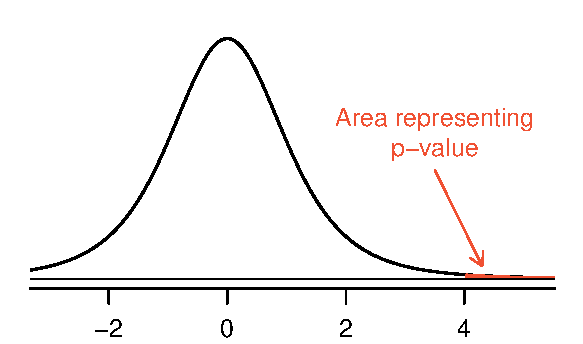
\includegraphics[width=0.6\textwidth]{06/figures/stemCellTherapyForHeartsPValue/stemCellTherapyForHeartsPValue}
\caption{Distribution of the sample difference of the mean improvements if the null hypothesis was true. The shaded area represents the p-value.}
\label{stemCellTherapyForHeartsPValue}
\end{figure}

\subsection{Two sample $t$ confidence interval}

Based on the results of Exercise~\exer{exerciseToEvaluteWhetherESCsAreHelpfulInImprovingHeartFunctionInSheep}, you found significant evidence that ESCs actually help improve the pumping function of the heart. But how large is this improvement? To answer this question, we can use a confidence interval. 

\begin{exercise}
In Exercise~\exer{exerciseToEvaluteWhetherESCsAreHelpfulInImprovingHeartFunctionInSheep}, you found that the point estimate, $\bar{x}_{esc} - \bar{x}_{control} = 7.88$, has a standard error of 1.95. Using $df=8$, create a 99\% confidence interval for the improvement due to ESCs. Answer in the footnote\footnote{We know the point estimate, 7.88, and the standard error, 1.95. We also verified the conditions for using the $t$ distribution in Exercise~\exer{exerciseToEvaluteWhetherESCsAreHelpfulInImprovingHeartFunctionInSheep}. Thus, we only need identify $t^{\star}_8$ to create a 99\% confidence interval: $t^{\star}_{8} = 3.36$. Thus, the 99\% confidence interval for the improvement from ESCs is given by $$7.88 \pm 3.36*1.95 \quad\to\quad (1.33, 14.43)$$ That is, we are 99\% confident that the true improvement in heart pumping function is somewhere between 1.33\% and 14.43\%.}.
\end{exercise}

\subsection{Pooled standard deviation estimate (special topic)}
\label{pooledStandardDeviations}

Occasionally, two populations will have standard deviations that are so similar, that they can be treated as identical. For example, historical data or a well-understood biological mechanism may justify this strong assumption. In such cases, we can make our $t$ distribution approach slightly more precise by using a pooled standard deviation.

The \term{pooled standard deviation} of two groups is a way to use data from both samples to better estimate the standard deviation and standard error. If $s_1^{}$ and $s_2^{}$ are the standard deviations of groups 1 and 2 and there are good reasons to believe that the population standard deviations are equal, then we can obtain an improved estimate of the group variances by pooling their data:
\begin{align*}
s_{pooled}^2 = \frac{s_1^2*(n_1-1) + s_2^2*(n_2-1)}{n_1 + n_2 - 2}
\end{align*}
where $n_1$ and $n_2$ are the sample sizes, as before. To utilize this new statistic, we substitute $s_{pooled}^2$ in place of $s_1^2$ and $s_2^2$ in the standard error formula, and we use an updated formula for the degrees of freedom:
\begin{align*}
df = n_1 + n_2 - 2
\end{align*}

The benefits of pooling the standard deviation are realized through obtaining a better estimate of the population standard deviations and using a larger degrees of freedom parameter for the $t$ distribution. Both of these changes may permit a better model of the sampling distribution of $\bar{x}_1^2 - \bar{x}_2^2$.

\begin{caution}
{Pooling standard deviations should be done only after careful research}
{A pooled standard deviation is only appropriate when background research indicates the population standard deviations are nearly equal. When the sample size is large and the condition may be adequately checked with data, the benefits of pooling the standard deviations greatly diminishes.}
\end{caution}

%As a general rule of thumb, we advise implementing the unequal standard deviation approach promoted earlier in this section unless there is strong reason to believe the standard deviations are equal. 
%However, we will find that pooled standard deviations are useful to a commonly used technique in Chapter~\ref{multipleRegressionAndANOVA} called analysis of variance (ANOVA).


%As a general rule of thumb, we advise against pooling standard deviations for the two-sample mean test due to the difficulty in. Verifying the assumption that the standard deviations are equal is difficult without a large sample, and in such cases, there is virtually no difference between using the standard estimates of standard deviation and using the pooled approach.




\section[Small sample hypothesis testing for a proportion (special topic)]{Small sample hypothesis testing for a proportion\\(special topic)}
\label{smallSampleHTForProportion}

In this section we develop inferential methods for a single proportion that are appropriate when the sample size is too small to apply the normal model to $\hat{p}$. Just like the other small sample techniques, the methods introduced here can be applied to large samples.

\subsection{When the success-failure condition is not met}

People providing an organ for donation sometimes seek the help of a special ``medical consultant''. These consultants assist the patient in all aspect of the surgery, with the goal of reducing the possibility of complications during the medical procedure and recovery. Patients might choose a consultant based in part on the historical complication rate of the consultant's clients. One consultant tried to attract patients by noting the average complication rate for liver donor surgeries in the US is about 10\%, but her clients have only had 3 complications in the 62 liver donor surgeries she has facilitated. She claims this is strong evidence that her work meaningfully contributes to reducing complications (and therefore she should be hired!).

\begin{exercise}
We will let $p$ represent the true complication rate for liver donors working with this consultant. Estimate $p$ using the data, and label this value $\hat{p}$.
\end{exercise}

\begin{example}{Is it possible to assess the consultant's claim using the data provided?}
No. The claim is that there is a causal connection, but the data are observational. Patients who hire this medical consultant may have lower complication rates for other reasons.

While it is not possible to assess this causal claim, it is still possible to test for an association using these data. For this question we ask, Could the low complication rate of $\hat{p} = 3/62=0.048$ be due to chance?
\end{example}

\begin{exercise} \label{hypForAssessingConsultantWorkInLiverTransplants}
Write out hypotheses in both plain and statistical language to test for the association between the consultant's work and the true complication rate, $p$, for this consultant's clients. Answer in the footnote\footnote{$H_0$: There is no association between the consultant's contributions and the clients' complication rate. In statistical language, $p=0.10$. $H_A$: Patients who work with the consultant tend to have a complication rate lower than 10\%, i.e. $p<0.10$.}.
\end{exercise}

\begin{example}{In the examples based on large sample theory, we modeled $\hat{p}$ using the normal distribution. Why is this not appropriate here?}
The independence assumption may be reasonable if each of the surgeries is from a different surgical team. However, the success-failure condition is not satisfied. Under the null hypothesis, we would anticipate seeing $62*0.10=6.2$ complications, not the 10 required for the normal approximation.
\end{example}

The uncertainty associated with the sample proportion should not be modeled using the normal distribution. However, we would still like to assess the hypotheses from Exercise~\ref{hypForAssessingConsultantWorkInLiverTransplants} in absence of the normal framework. To do so, we need to evaluate the possibility of a sample value ($\hat{p}$) this far below the null value, $p_0=0.10$. This possibility is usually measured with a p-value.

The p-value is computed based on the null distribution, which is the distribution of the test statistic if the null hypothesis is true. Supposing the the null hypothesis is true, we can compute the p-value by identifying the chance of observing a test statistic that favors the alternative hypothesis at least as strongly as the observed test statistic. In other words, we compute the tail area (or areas) to identify the p-value.

\subsection{Generating the null distribution and p-value by simulation}
\label{generatingTheNullDistributionAndPValueBySimulationForOneProportion}

We want to identify the sampling distribution of the test statistic ($\hat{p}$) if the null hypothesis was true. In other words, we want to see how the sample proportion changes due to chance alone. Then we plan to use this information to decide whether there is enough evidence to reject the null hypothesis.

Under the null hypothesis, 10\% of liver donors have complications during or after surgery. Suppose this rate was really no different for the consultant's clients. If this was the case, we could \emph{simulate} 62 clients to get a sample proportion for the complication rate from the null distribution.

Each client can be simulated using a deck of cards. Take one red card, nine black cards, and mix them up. Then drawing a card is one way of simulating the chance a patient has a complication \emph{if the true complication rate is 10\%} for the data. If we do this 62 times and compute the proportion of patients with complications in the simulation, $\hat{p}_{sim}$, then this sample proportion is exactly a sample from the null distribution.

An undergraduate student was paid \$2 to complete this simulation. There were 5 simulated cases with a complication and 57 simulated cases without a complication, i.e. $\hat{p}_{sim} = 5/62 = 0.081$.

\begin{example}{Is this one simulation enough to determine whether or not we should reject the null hypothesis from Exercise~\ref{hypForAssessingConsultantWorkInLiverTransplants}? Explain.}
No. To assess the hypotheses, we need to see a distribution of many $\hat{p}_{sim}$, not just a \emph{single} draw from this sampling distribution.
\end{example}

One simulation isn't enough to get a sense of the null distribution; many simulation studies are needed. Roughly 10,000 seems sufficient. However, paying someone to simulate 10,000 studies by hand is a waste of time and money. Instead, simulations are typically programmed into a computer, which is fast and cheap.

Figure~\ref{nullDistForPHatIfLiverTransplantConsultantIsNotHelpful} shows the results of 10,000 simulated studies. The proportions that are equal to or less than $\hat{p}=0.048$ are shaded. The shaded areas represent sample proportions under the null distribution that provide at least as much evidence as $\hat{p}$ favoring the alternative hypothesis. There were 1222 simulated sample proportions with $\hat{p}_{sim} \leq 0.048$. We use these to construct the null distribution's left-tail area and find the p-value:
\begin{align}
\text{left tail }\label{estOfPValueBasedOnSimulatedNullForSingleProportion}
	&= \frac{\text{Number of observed simulations with }\hat{p}_{sim}\leq\text{ 0.048}}{10000}
\end{align}
Of the 10,000 simulated $\hat{p}_{sim}$, 1222 were equal to or smaller than $\hat{p}$. Since the hypothesis test is one-sided, the estimated p-value is equal to this tail area: 0.1222.
\begin{figure}
\centering
\includegraphics[width=0.9\textwidth]{06/figures/nullDistForPHatIfLiverTransplantConsultantIsNotHelpful/nullDistForPHatIfLiverTransplantConsultantIsNotHelpful}
\caption{The null distribution for $\hat{p}$, created from 10,000 simulated studies. The left tail, representing the p-value for the hypothesis test, contains 12.22\% of the simulations.}
\label{nullDistForPHatIfLiverTransplantConsultantIsNotHelpful}
\end{figure}

\begin{exercise} \label{rejectOrNotForHTForLiverDonorSurgicalConsultant}
Based on the estimated p-value of 0.1222, should the null hypothesis be rejected? Give a brief explanation.
\end{exercise}

\begin{exercise} \label{plainLanguageExplanationOfHTConclusionForLiverDonorSurgicalConsultant}
Because the estimated p-value is 0.1222, which is larger than the significance level 0.05, we do not reject the null hypothesis. Explain what this means in plain language in the context of the problem. Answer in the footnote\footnote{There isn't sufficiently strong evidence to support an association between the consultant's work and fewer surgery complications.}.
\end{exercise}

\begin{exercise}
Does the conclusion in Exercise~\ref{plainLanguageExplanationOfHTConclusionForLiverDonorSurgicalConsultant} imply there is no real association between the surgical consultant's work and fewer complications? Explain. Answer in the footnote\footnote{No. It might be that the consultant's work is associated with a reduction but that there isn't enough data to convincingly show this connection.}.
\end{exercise}

\begin{termBox}{\tBoxTitle{One-sided hypothesis test for $p$ with a small sample}
The p-value is always derived by analyzing the null distribution of the test statistic. The normal model poorly approximates the null distribution for $\hat{p}$ when the success-failure condition is not satisfied. As a substitute, we generate the null distribution using simulated sample proportions ($\hat{p}_{sim}$) and use this distribution to compute the tail area, i.e. the p-value.}
\end{termBox}

How do we compute the p-value when the test is two-sided? We continue to use the same rule as before: double the single tail area, which remains a reasonable approach even when the sampling distribution is assymmetric. However, this can result in p-values larger than 1 when the point estimate is very near the mean in the null distribution; in such cases, we write that the p-value is 1. Also, very large p-values computed in this way (e.g. 0.85), may also be slightly inflated.

%How do we compute the p-value when the test is two-sided? One reasonable approach is to identify the difference of the point estimate and the null value ($|\hat{p} - p_0|$), then add up all areas that are at least this far from the null value. A second approach uses the rule derived from the symmetric distribution case: double the single tail area. However, this second way to describe the p-value can result in p-values larger than zero when the point estimate is very near the null value in the null distribution (in such cases, we write that the p-value is one). These two methods for computing p-values will not always agree. The first approach is ideal

Exercises~\ref{rejectOrNotForHTForLiverDonorSurgicalConsultant} and~\ref{plainLanguageExplanationOfHTConclusionForLiverDonorSurgicalConsultant} said the p-value is \emph{estimated}. It is not exact because the simulated null distribution itself is not exact, only a close approximation. However, we can generate an exact null distribution and p-value using the binomial model from Section~\ref{binomialModel}.

\subsection{Generating the exact null distribution and p-value}
\label{exactNullDistributionUsingBinomialModel}

The number of successes in $n$ independent cases can be described using the binomial model, which was introduced in Section~3.4%ZZQ \ref{}
. Recall that the probability of observing exactly $k$ successes is given by
\begin{align} \label{binomialEquationShownForFindingNullDistributionInSmallSamplePropTest}
P(k\text{ successes}) = {n\choose k} p^{k}(1-p)^{n-k} = \frac{n!}{k!(n-k)!} p^{k}(1-p)^{n-k}
\end{align}
where $p$ is the true probability of success. The expression ${n\choose k}$ is read as \emph{$n$ choose $k$}, and the exclamation points represent factorials. For instance, $3!$ is equal to $3*2*1=6$, $4!$ is equal to $4*3*2*1 = 24$, and so on (see Section~3.4%ZZQ \ref{}
).

The tail area of the null distribution is computed by adding up the probability in Equation~\eqref{binomialEquationShownForFindingNullDistributionInSmallSamplePropTest} for each $k$ that provides at least as strong of evidence favoring the alternative hypothesis as the data. If the hypothesis test is one-sided, then the p-value is represented by a single tail area. If the test is two-sided, compute the single tail area and double it to get the p-value, just as we have done in the past.

\begin{example}{Compute the exact p-value to check the consultant's claim that her clients' complication rate is below 10\%.}
Exactly $k=3$ complications were observed in the $n=62$ cases cited by the consultant. Since we are testing against the 10\% national average, our null hypothesis is $p=0.10$. We can compute the p-value by adding up the cases where there are 3 or fewer complications:
\begin{align*}
\text{p-value}
	&= \sum_{j=0}^{3} {n\choose j} p^{j}(1-p)^{n-j} \\
	&= \sum_{j=0}^{3} {62\choose j} 0.1^{j}(1-0.1)^{62-j} \\
	&= {62\choose 0} 0.1^{0}(1-0.1)^{62-0} +
		{62\choose 1} 0.1^{1}(1-0.1)^{62-1} \\
	& \qquad + {62\choose 2} 0.1^{2}(1-0.1)^{62-2} +
		{62\choose 3} 0.1^{3}(1-0.1)^{62-3} \\
	&= 0.0015 + 0.0100 + 0.0340 + 0.0755 \\
	&= 0.1210
\end{align*}
This exact p-value is very close to the p-value based on the simulations (0.1222), and we come to the same conclusion. We do not reject the null hypothesis, and there is not statistically significant evidence to support the association.

If it were plotted, the exact null distribution would look almost identical to the simulated null distribution shown in Figure~\ref{nullDistForPHatIfLiverTransplantConsultantIsNotHelpful} on page~\pageref{nullDistForPHatIfLiverTransplantConsultantIsNotHelpful}.
\end{example}


\section[Hypothesis testing for two proportions (special topic)]{Hypothesis testing for two proportions \\ (special topic)}
\label{smallSampleHTForTwoOrMoreProportion}

%Data: Bottiger2001. 90 patients had received CPR outside of a hospital premises, and investigators wanted to determine whether thrombolytic therapy (treatment to dissolve blood clots) was beneficial to patients in survival. There is concern that this treatment may complicate any internal bleeding resulting from CPR. Of the 90 patients who entered the study, 50 were in the control group and 40 in treatment group. After 24 hours, 11 patients in the control group and 14 in the treatment group were still alive.
%\begin{itemize}\color{gray}
%\item[6.1] Describe the problem
%\item[6.1] Point out that we could apply large sample methods, but this is a border case. Furthermore, the number of successes and failures in all categories is relatively small, so we may like to investigate this more carefully.
%\item[6.2] Present the randomization idea from Section 1.6
%\item[6.2] Simulate one fake result
%\item[6.2] Simulate many results, creating the null distribution
%\item[6.2] Describe the conclusion
%\end{itemize}

Cardiopulmonary resuscitation (CPR) is a procedure commonly used on individuals suffering a heart attack when other emergency resources are not available. This procedure is helpful in maintaining some blood circulation, but the chest compressions involved can also cause internal injuries. Internal bleeding and other injuries complicate additional treatment efforts following arrival at a hospital. For instance, blood thinners may be used to help release a clot that is causing the heart attack. However, the blood thinner would have negative repercussions on any internal injuries. Here we consider an experiment\footnote{\emph{Efficacy and safety of thrombolytic therapy after initially unsuccessful cardiopulmonary resuscitation: a prospective clinical trial}, by B$\ddot{\text{o}}$ttiger et al., The Lancet, 2001.} for patients who underwent CPR for a heart attack and were subsequently admitted to a hospital. These patients were randomly divided into a treatment group where they received a blood thinner or the control group where they did not receive the blood thinner. The outcome variable of interest was whether the patients survived for at least 24 hours.

\begin{example}{Form hypotheses for this study in plain and statistical language. Let $p_c$ represent the true survival proportion in the control group and $p_t$ represent the survival proportion for the treatment group.} \label{hypothesesForCPRStudyInSmallSampleSection}
We are interested in whether the blood thinners are helpful or hurtful, so this should be a two-sided test.
\begin{itemize}
\item[$H_0$:] Blood thinners do not have an overall effect on survival, i.e. the survival proportions are the same in each group. $p_t - p_c = 0$.
\item[$H_A$:] Blood thinners do have an impact on survival. $p_t - p_c \neq 0$.
\end{itemize}
\end{example}

\subsection{Large sample framework for a difference in two proportions}

There were 50 patients in the experiment who did not receive the blood thinner and 40 patients who did. The study results are shown in Table~\ref{resultsForCPRStudyInSmallSampleSection}.

\begin{table}[ht]
\centering
\begin{tabular}{lccccc}
\hline
			&& Survived 	& Died 	&& Total \\
\hline
Control		&& 11		& 39		&& 50 \\
Treatment		&& 14		& 26		&& 40 \\
\hline
Total			&& 25		& 65		&& 90 \\
\hline
\end{tabular}
\caption{Results for the CPR study. Patients in the treatment group were given a blood thinner, and patients in the control group were not.}
\label{resultsForCPRStudyInSmallSampleSection}
\end{table}

\begin{exercise}
What is the sample survival proportion of the control group? Of the treatment group? Provide a point estimate of the difference in survival proportions of the two groups: $\hat{p}_t - \hat{p}_c$. Answer in the footnote\footnote{$\hat{p}_t - \hat{p}_c = 0.35 - 0.22 = 0.13$}.
\end{exercise}

According to the point estimate, there is a 13\% increase in the survival proportion when patients who have undergone CPR outside of the hospital are treated with blood thinners. However, we wonder if this difference could be due to chance. We'd like to investigate this using a large sample framework, but we first need to check the conditions for such an approach.

%ZZQ Formatting
\pagebreak

\begin{example}{Can the point estimate of the difference in survival proportions be adequately modeled using a normal distribution?}
We will assume the patients are independent, which is probably reasonable. The success-failure condition is also satisfied. There were at least 10 successes and 10 failures in each group.
\end{example}

While we can apply a normal framework as an approximation to find a p-value, we might keep in mind that there were just 11 successes in one group and 14 in the other. Below we conduct an analysis relying on the large sample normal theory. We will follow up with a small sample analysis and compare the results.

\begin{example}{Assess the hypotheses presented in Example~\ref{hypothesesForCPRStudyInSmallSampleSection} using a large sample framework. Use a significance level of $\alpha=0.05$.}
We suppose the null distribution of the sample difference follows a normal distribution with mean 0 (the null value) and a standard deviation equal to the standard error of the estimate. Because the null hypothesis in this case would be that the two proportions are the same, we compute the standard error using the pooled standard error formula from Equation~\eqref{seOfDiffInPropUsingPooledEstimate} on page~\pageref{seOfDiffInPropUsingPooledEstimate}:
\begin{align*}
SE = \sqrt{\frac{p(1-p)}{n_t} + \frac{p(1-p)}{n_c}}
	\approx \sqrt{\frac{0.278(1-0.278)}{40} + \frac{0.278(1-0.278)}{50}} = 0.095
\end{align*}
where we have used the pooled estimate $\left( \hat{p} = \frac{11+14}{50 + 40} = 0.278 \right)$ in place of the true proportion, $p$.

The null distribution with mean zero and standard deviation 0.095 is shown in Figure~\ref{pValueCPRStudyLargeSampleAnalysisInSmallSampleSection}. We compute the tail areas to identify the p-value. To do so, we use the Z score of the point estimate:
\begin{align*}
Z = \frac{(\hat{p}_t - \hat{p}_c) - \text{null value}}{SE} = \frac{0.13 - 0}{0.095} = 1.37
\end{align*}
If we look this Z score up in Appendix~\ref{normalProbabilityTable}, we see that the right tail has area 0.0853. The p-value is twice the single tail area: 0.176. This p-value does not provide convincing evidence that the blood thinner helps. Thus, there is insufficient evidence to conclude whether or not the blood thinner helps or hurts. (Remember, we never ``accept'' the null hypothesis -- we can only reject or fail to reject.)
\end{example}
\begin{figure}[ht]
\centering
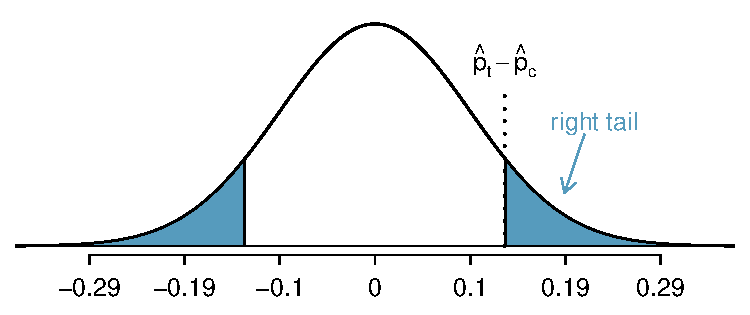
\includegraphics[width=0.75\textwidth]{06/figures/pValueCPRStudyLargeSampleAnalysisInSmallSampleSection/pValueCPRStudyLargeSampleAnalysisInSmallSampleSection}
\caption{The null distribution of the point estimate, $\hat{p}_t - \hat{p}_c$, under the large sample framework is a normal distribution with mean $0$ and standard deviation equal to the standard error, in this case $SE=0.095$. The p-value is represented as sample differences in the null distribution that provide greater evidence for the alternative hypothesis than what the observed data present. The p-value is represented by the shaded areas.}
\label{pValueCPRStudyLargeSampleAnalysisInSmallSampleSection}
\end{figure}

The p-value given here, 0.176, relies on the normal approximation. We know that as the samples sizes are large, this approximation is quite good. However, when the sample sizes are relatively small -- the success failure condition is either not satisfied or is just barely satisfied -- the approximation may only be adequate. Next we develop a small sample technique, apply it to these data, and compare our results. In general, the small sample method we develop may be used for any size sample, small or large, and should be considered as more accurate than the corresponding large sample technique.

\subsection{Simulating a difference under the null distribution}

The ideas in this section were first introduced in the optional Section~\ref{caseStudyOfSulphinpyrazone} on page~\pageref{caseStudyOfSulphinpyrazone}. For the interested reader, this earlier section provides a more in-depth discussion.

Suppose the null hypothesis is true. Then the blood thinner has no impact on survival and the 13\% difference was due to chance. In this case, we can simulate \emph{null} differences that are due to chance using a \emph{randomization technique}\footnote{The test procedure we employ in this section is formally called a \term{permutation test}.}. By randomly assigning ``fake treatment'' and ``fake control'' stickers to the patients' files, we could get a new grouping -- one that is completely due to chance. The expected difference between the two proportions under this simulation is zero.

We run this simulation by taking 40 \resp{treatmentFake} and 50 \resp{controlFake} labels and randomly assigning them to the patients. The label counts of 40 and 50 correspond to the number of treatment and control assignments in the actual study. We use a computer program to randomly assign these labels to the patients, and we organize the simulation results into Table~\ref{resultsForCPRStudyInSmallSampleSectionFake1}.
\begin{table}[ht]
\centering
\begin{tabular}{lccccc}
\hline
			&& Survived 	& Died 	&& Total \\
\hline
\resp{controlFake}		&& 15		& 35		&& 50 \\
\resp{treatmentFake}	&& 10		& 30		&& 40 \\
\hline
Total			&& 25		& 65		&& 90 \\
\hline
\end{tabular}
\caption{Simulated results for the CPR study under the null hypothesis. The labels were randomly assigned and are independent of the outcome of the patient.}
\label{resultsForCPRStudyInSmallSampleSectionFake1}
\end{table}

\begin{exercise} \label{exerciseComputingDifferenceForCPRStudyInSmallSampleSectionFake1}
What is the difference in death rates between the two fake groups in Table~\ref{resultsForCPRStudyInSmallSampleSectionFake1}? How does this compare to the observed 13\% in the real groups?
\end{exercise}

The difference computed in Exercise~\ref{exerciseComputingDifferenceForCPRStudyInSmallSampleSectionFake1} represents a draw from the null distribution of the sample differences. Next we generate many more simulations to build up the null distribution, much like we did in Section~\ref{generatingTheNullDistributionAndPValueBySimulationForOneProportion} to build a null distribution for one sample proportion.

\begin{caution}{Simulation in the two proportion case requires that the null difference is zero}
{The technique described here to simulate a difference from the null distribution relies on an important condition in the null hypothesis: there is no connection between the two variables considered. In some special cases, the null difference might not be zero, and more advanced methods (or a large sample approximation, if appropriate) would be necessary.}
\end{caution}

\subsection{Null distribution for the difference in two proportions}

We build up an approximation to the null distribution by repeatedly creating tables like the one shown in Table~\ref{resultsForCPRStudyInSmallSampleSectionFake1} and computing the sample differences. The null distribution from 10,000 simulations is shown in Figure~\ref{pValueCPRStudySmallSampleAnalysisInSmallSampleSection}.
\begin{figure}
\centering
\includegraphics[width=0.78\textwidth]{06/figures/pValueCPRStudySmallSampleAnalysisInSmallSampleSection/pValueCPRStudySmallSampleAnalysisInSmallSampleSection}
\caption{An approximation of the null distribution of the point estimate, $\hat{p}_t - \hat{p}_c$. The p-value is twice the right tail area.} %represented as the areas at least as far from the null value as what was observed.}
\label{pValueCPRStudySmallSampleAnalysisInSmallSampleSection}
\end{figure}

\begin{example}{Compare Figures~\ref{pValueCPRStudyLargeSampleAnalysisInSmallSampleSection} and~\ref{pValueCPRStudySmallSampleAnalysisInSmallSampleSection}. How are they similar? How are they different?}
The shapes are similar, but the simulated results show that the continuous approximation of the normal distribution is not very good. We might wonder, how close are the p-values?
\end{example}

\begin{exercise}
The right tail area is about 0.13. (It is only a coincidence that we also have $\hat{p}_t - \hat{p}_c=0.13$.) Since this is a two-sided test, what is the p-value?
\end{exercise}

\begin{exercise} \label{comparisonOfLargeSampleAndSmallSamplePValueInCPRStudy}
The p-value is computed by doubling the right tail area: 0.26. How does this value compare with the large sample approximation for the p-value? Answer in the footnote\footnote{The approximation in this case is fairly poor (p-values: 0.174 vs. 0.26), though we come to the same conclusion. The data do not provide convincing evidence showing the blood thinner hurts or helps patients.}.
\end{exercise}

%The large sample and small sample methods can give somewhat different results when the sample is somewhat small and the p-value is fairly large. So while the p-values in Exercise~\ref{comparisonOfLargeSampleAndSmallSamplePValueInCPRStudy} are quite a bit different, the differences would probably be a bit closer if the p-values were closer to zero.

%The large sample and small sample methods tend to give somewhat different results when the p-value is fairly large -- unless the conditions are not satisfied for large sample inference, then all bets are off. So while the p-values in Exercise~\ref{comparisonOfLargeSampleAndSmallSamplePValueInCPRStudy} are quite a bit different, the differences would probably be a bit closer if the p-values were closer to zero.

In general, small sample methods produce more accurate results since they rely on fewer assumptions. However, they often require some extra work or simulations. For this reason, many statisticians use small sample methods only when conditions for large sample methods are not satisfied.










